\chapter{Data}

\section{Probability Distibution to Find Particles $P(x)$}

\begin{figure}
  \centering
  \begin{subfigure}{.45\textwidth}
    \centering
    \includegraphics[width=\textwidth]{./data/plots/distrib-mit.pdf}
    \caption{With Laser, $\sigma = \num{0.1351}^{+0.0049}_{-0.0046}\si{\um}$}
  \end{subfigure}
  \begin{subfigure}{.45\textwidth}
    \centering
    \includegraphics[width=\textwidth]{./data/plots/distrib-ohne.pdf}
    \caption{Without Laser, $\sigma = \num{0.0771}^{+0.0028}_{-0.0026}\si{\um}$}
  \end{subfigure}
  \caption[Particle Distibution]{\textbf{Particle Distibution}, single particle each, 402 points at 13 fps}
\end{figure}

\begin{figure}
  \centering
  \includegraphics[width=\textwidth]{./data/plots/mostly-linear-fit.pdf}
  \caption{This should be linear, $m = \SI{1.403e-03}{\um\squared\per\second}$}
\end{figure}

Multiple free particles are located on the microscope slide and a \num{30} second video clip is recorded.
The free sofware \texttt{Blender} is used to track the motion of the particles and save the positions for later evaluation as the provided software sucks. \todo{rephrase}
The aquired positions are used to find the diffusion coefficient $D$ as established in \autoref{sec:brown}


\section{ink stuff}
A slide is prepared with a line of red and black felt-tip marker, alcohol is added as a solvent.
The slide is placed under the microscope and the laser is turned on on it's highest power setting.
Different effects are observed for both colors.

The black marker stripe looks uniform before turning on the laser.
The areas hit by the laser become lighter that their surroundings, the laser can be used to draw shapes.

The red marker stripe is not uniform, the pigment is distributed in a cell-like structure.
Turning on the laser causes the individual cells to merge.

\begin{figure}
  \centering
  \begin{subfigure}{.45\textwidth}
    \centering
    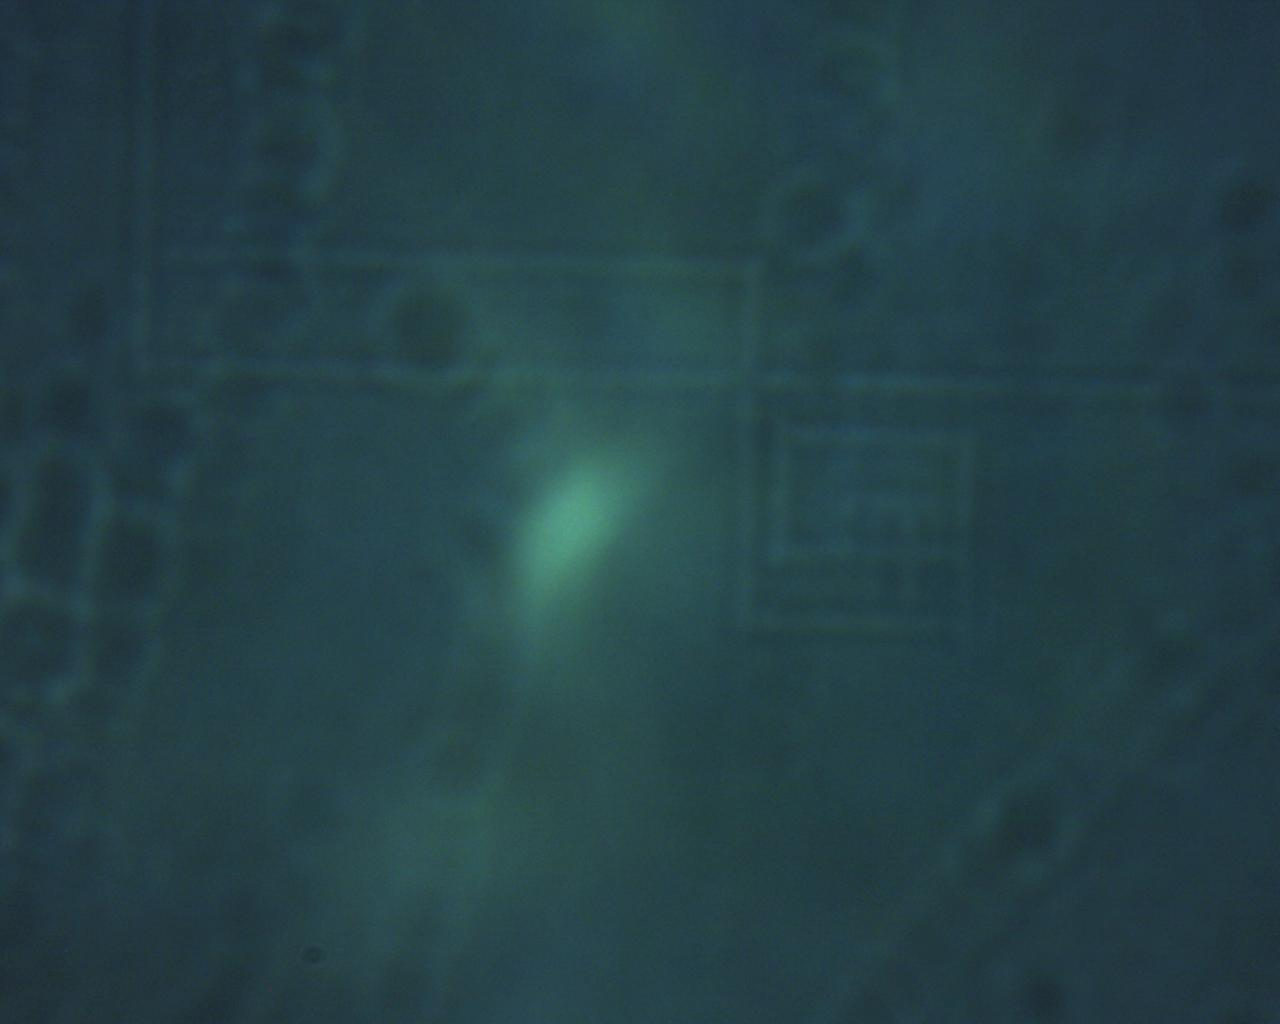
\includegraphics[width=\textwidth]{./data/source/schwarz.jpg}
    \caption{black permanent marker with spiral pattern drawn by laser}
  \end{subfigure}
  \begin{subfigure}{.45\textwidth}
    \centering
    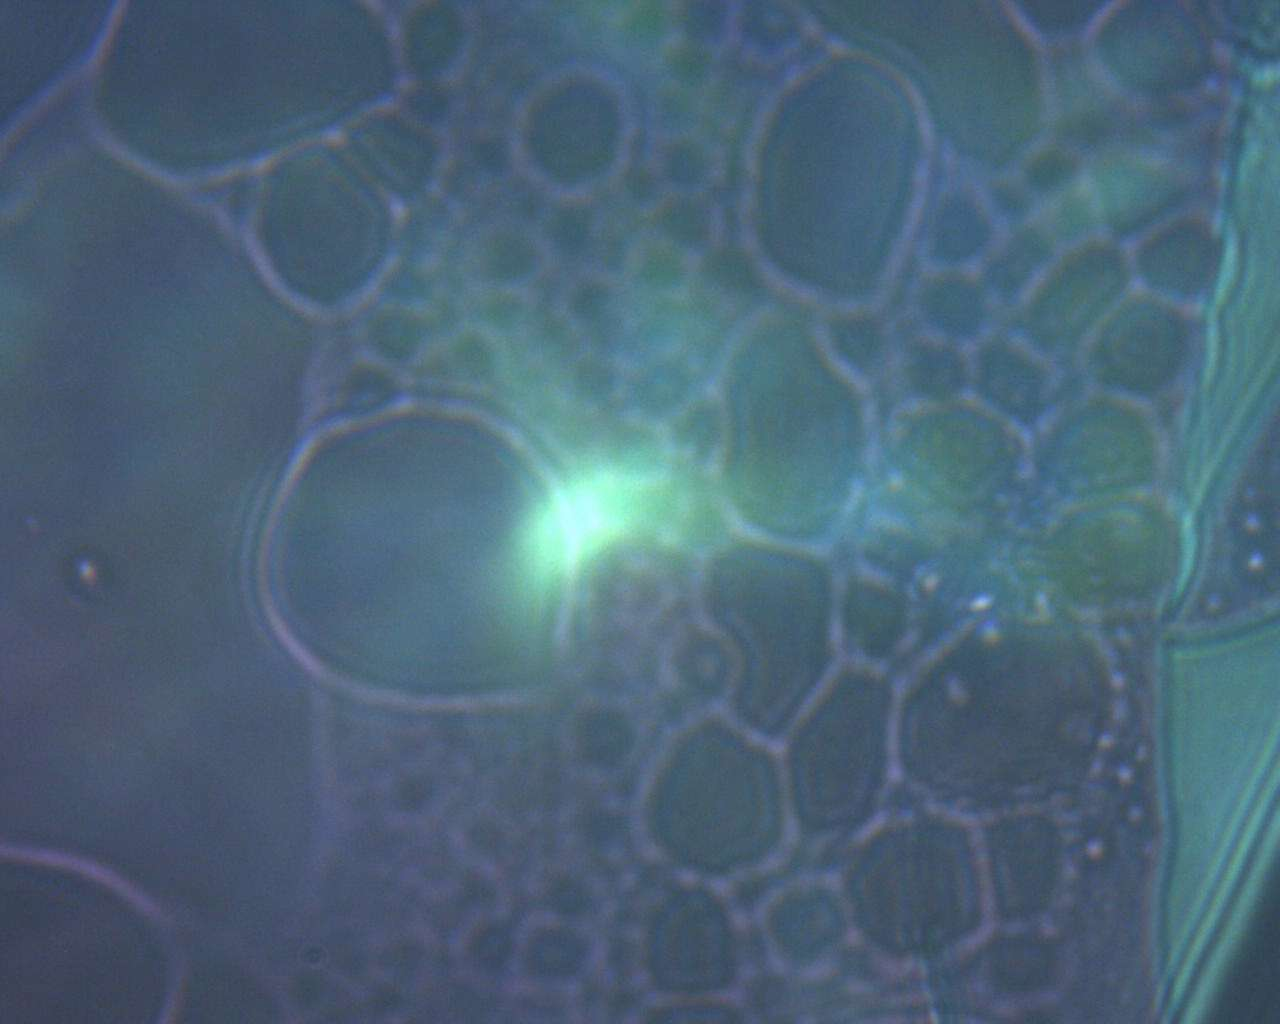
\includegraphics[width=\textwidth]{./img/red-before.jpg}
    \caption{red dry-erase marker before turning on the laser}
  \end{subfigure}
  \begin{subfigure}{.45\textwidth}
    \centering
    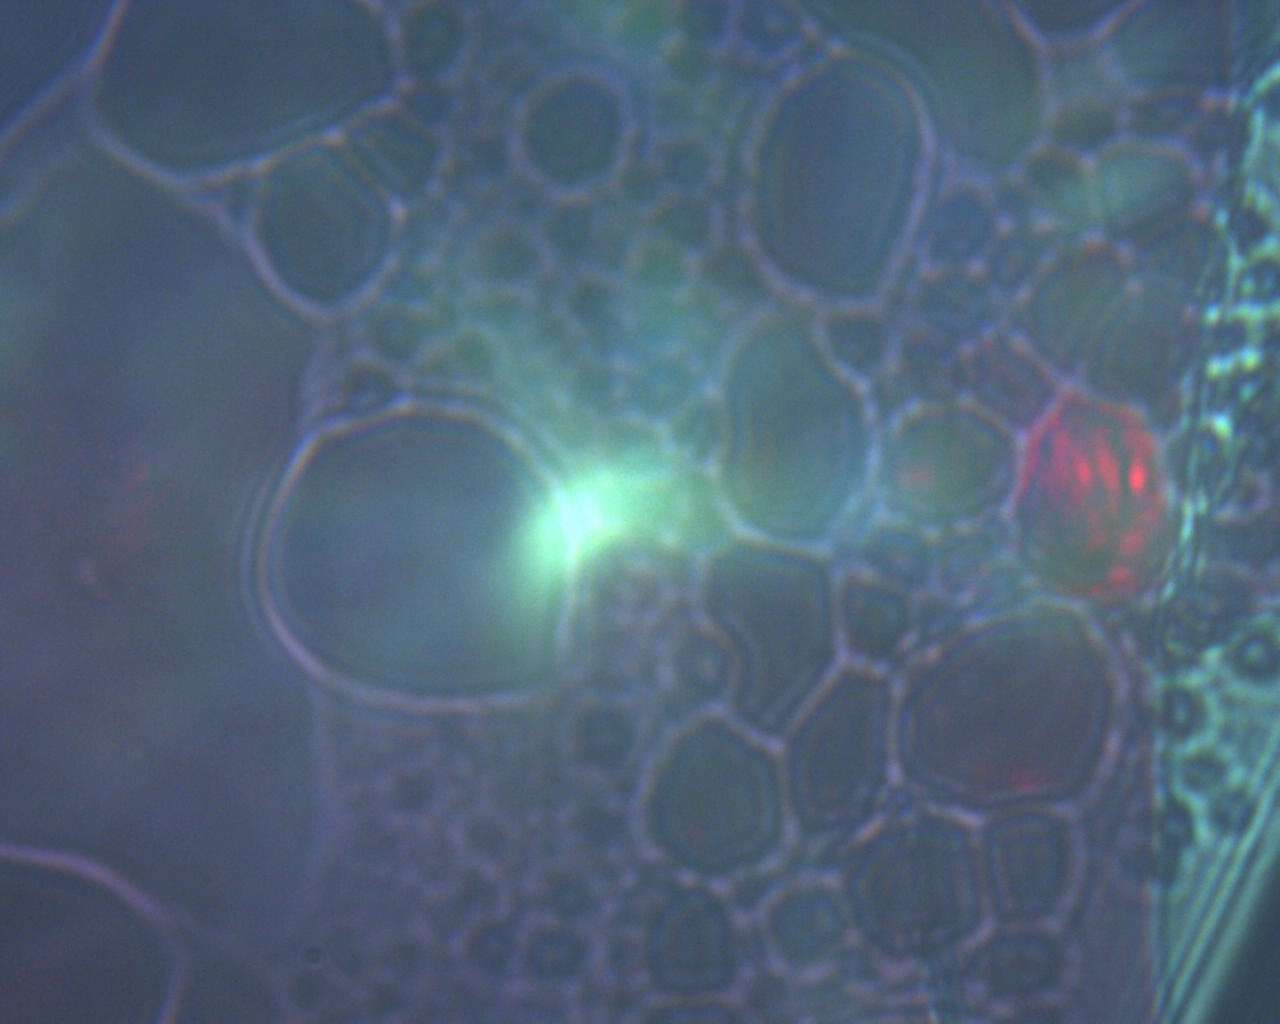
\includegraphics[width=\textwidth]{./img/red-1.jpg}
    \caption{red dry-erase marker immediately after turning on the laser}
  \end{subfigure}
  \begin{subfigure}{.45\textwidth}
    \centering
    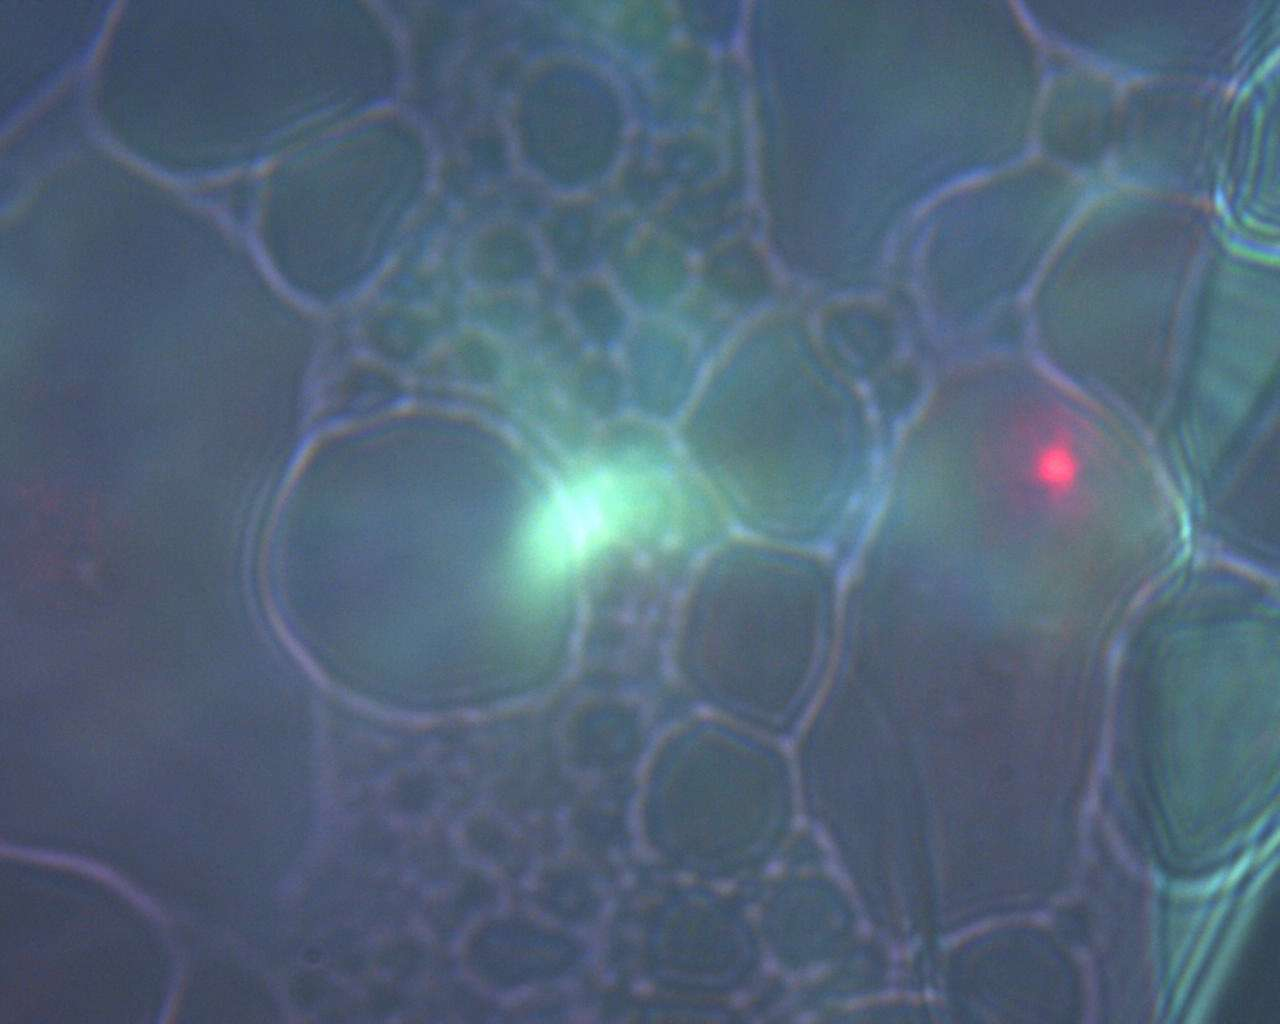
\includegraphics[width=\textwidth]{./img/red-2.jpg}
    \caption{red dry-erase marker \SI{\approx 20}{\s} after turning on the laser}
  \end{subfigure}

  \caption[Ink under laser]{\textbf{Ink under laser}, \num{114} microns across full width}
\end{figure}
